\maketitle

\section{Introduction}

\begin{frame}[fragile]{Motivation}
\centering
\only<1>{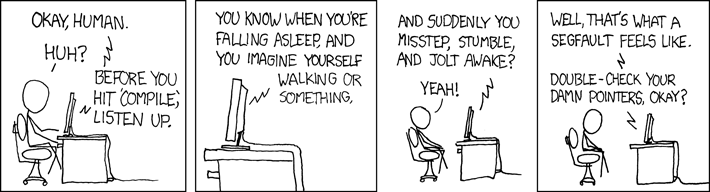
\includegraphics[width=\textwidth]{img/compiler_complaint.png}}

\only<2>{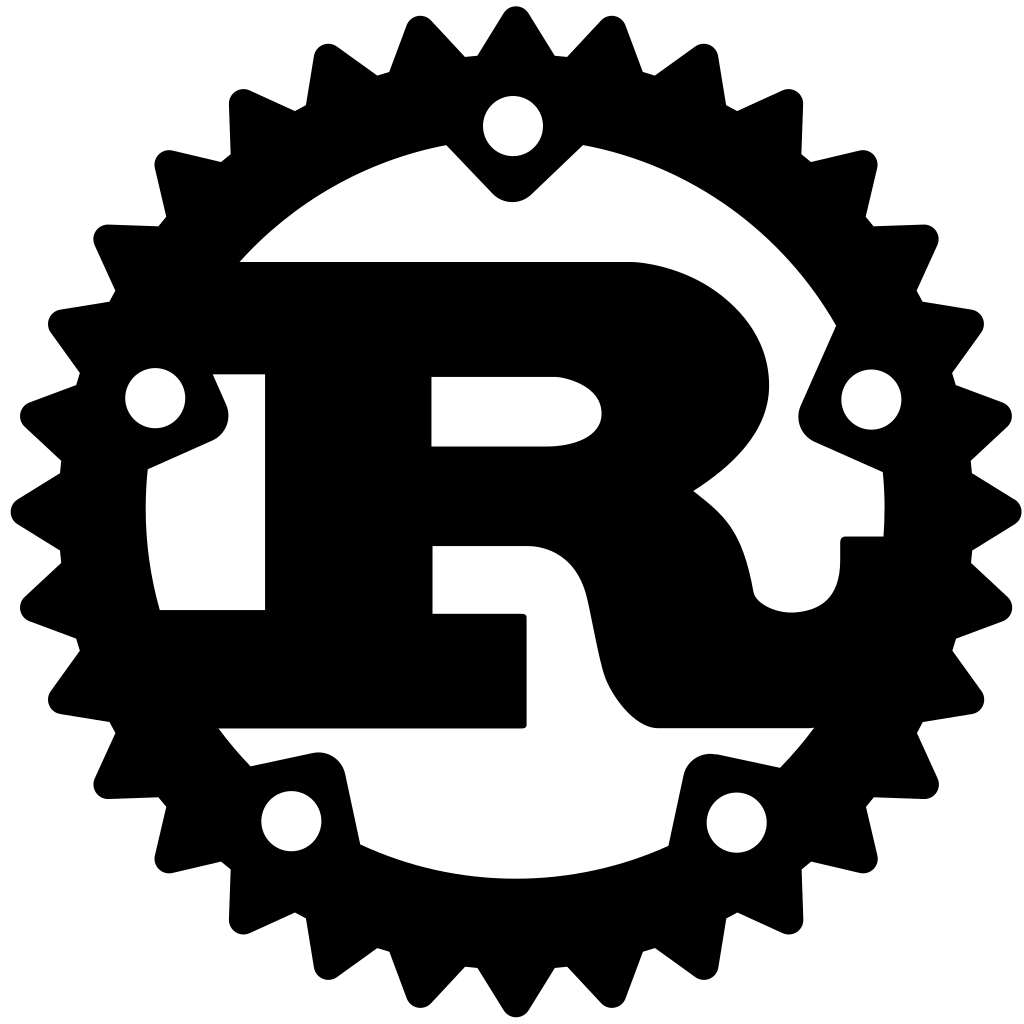
\includegraphics[width=0.3\textwidth]{img/rust.png}}

\begin{onlyenv}<3>
\begin{lstlisting}[style=short, language=Rust]
/// Returns the square of `x`. Squares are non-negative.
fn square(x: i32) -> i32 { -2 * x }
\end{lstlisting}
\end{onlyenv}

\begin{onlyenv}<4>
\begin{lstlisting}[style=short, language=Rust]
/// Returns the square of `x`. Squares are non-negative.
#[post(ret >= 0)]
fn square(x: i32) -> i32 { -2 * x }
// postcondition INVALID
\end{lstlisting}
\end{onlyenv}
\end{frame}


\begin{frame}{Presenting our tool}
  \begin{columns}
  \column{0.5\textwidth}
  \centering
  \Large{\texttt{rust-stainless}}

  \column{0.5\textwidth}
  \centering
  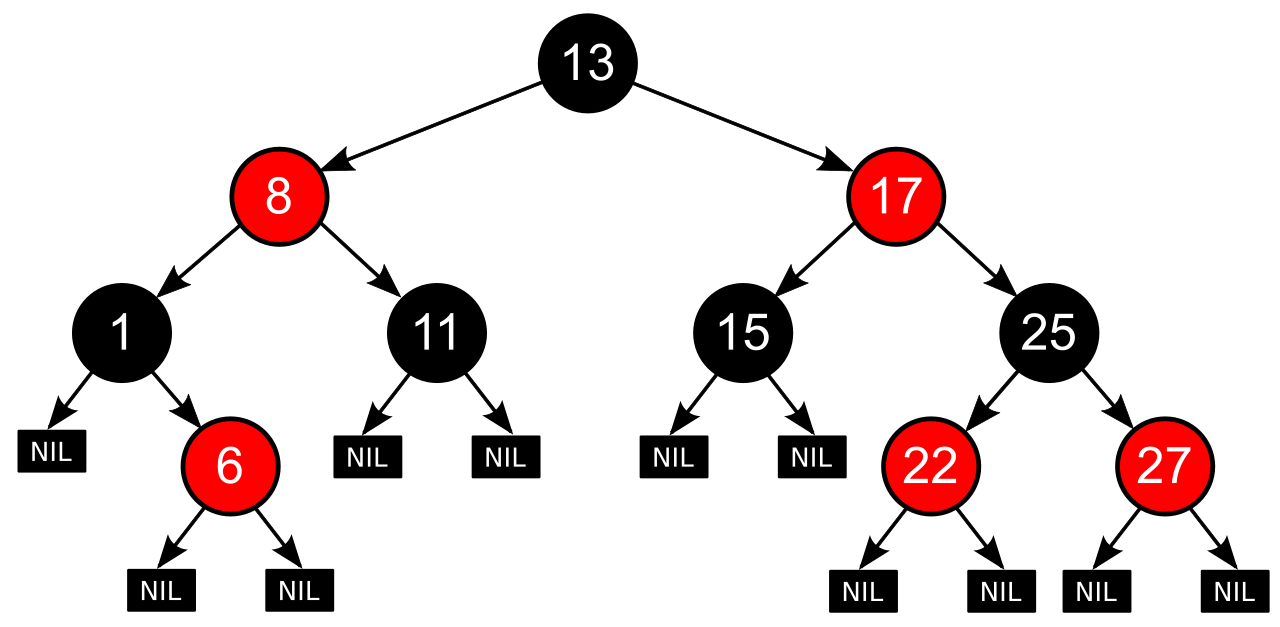
\includegraphics[width=\textwidth]{img/rbtree.png}
\end{columns}
\end{frame}


\begin{frame}{Contents}
  \setbeamertemplate{section in toc}[sections numbered]

  \tableofcontents%[hideallsubsections]
\end{frame}

\section{Verifying a Red-Black Tree}

\begin{frame}{Red-Black Tree}
\begin{columns}[T]
\column{0.5\textwidth}
\begin{itemize}
  \item Binary search tree
  \only<2->{
    \item Lookup, insertion and deletion in $\mathcal{O}(\log n)$ time
    \item But only if well balanced
  }
  \only<3->{
    \item Red-Black Tree uses colouring to automatically rebalance at insertion
    and deletion
  }
\end{itemize}

\column{0.5\textwidth}
\centering
\only<1>{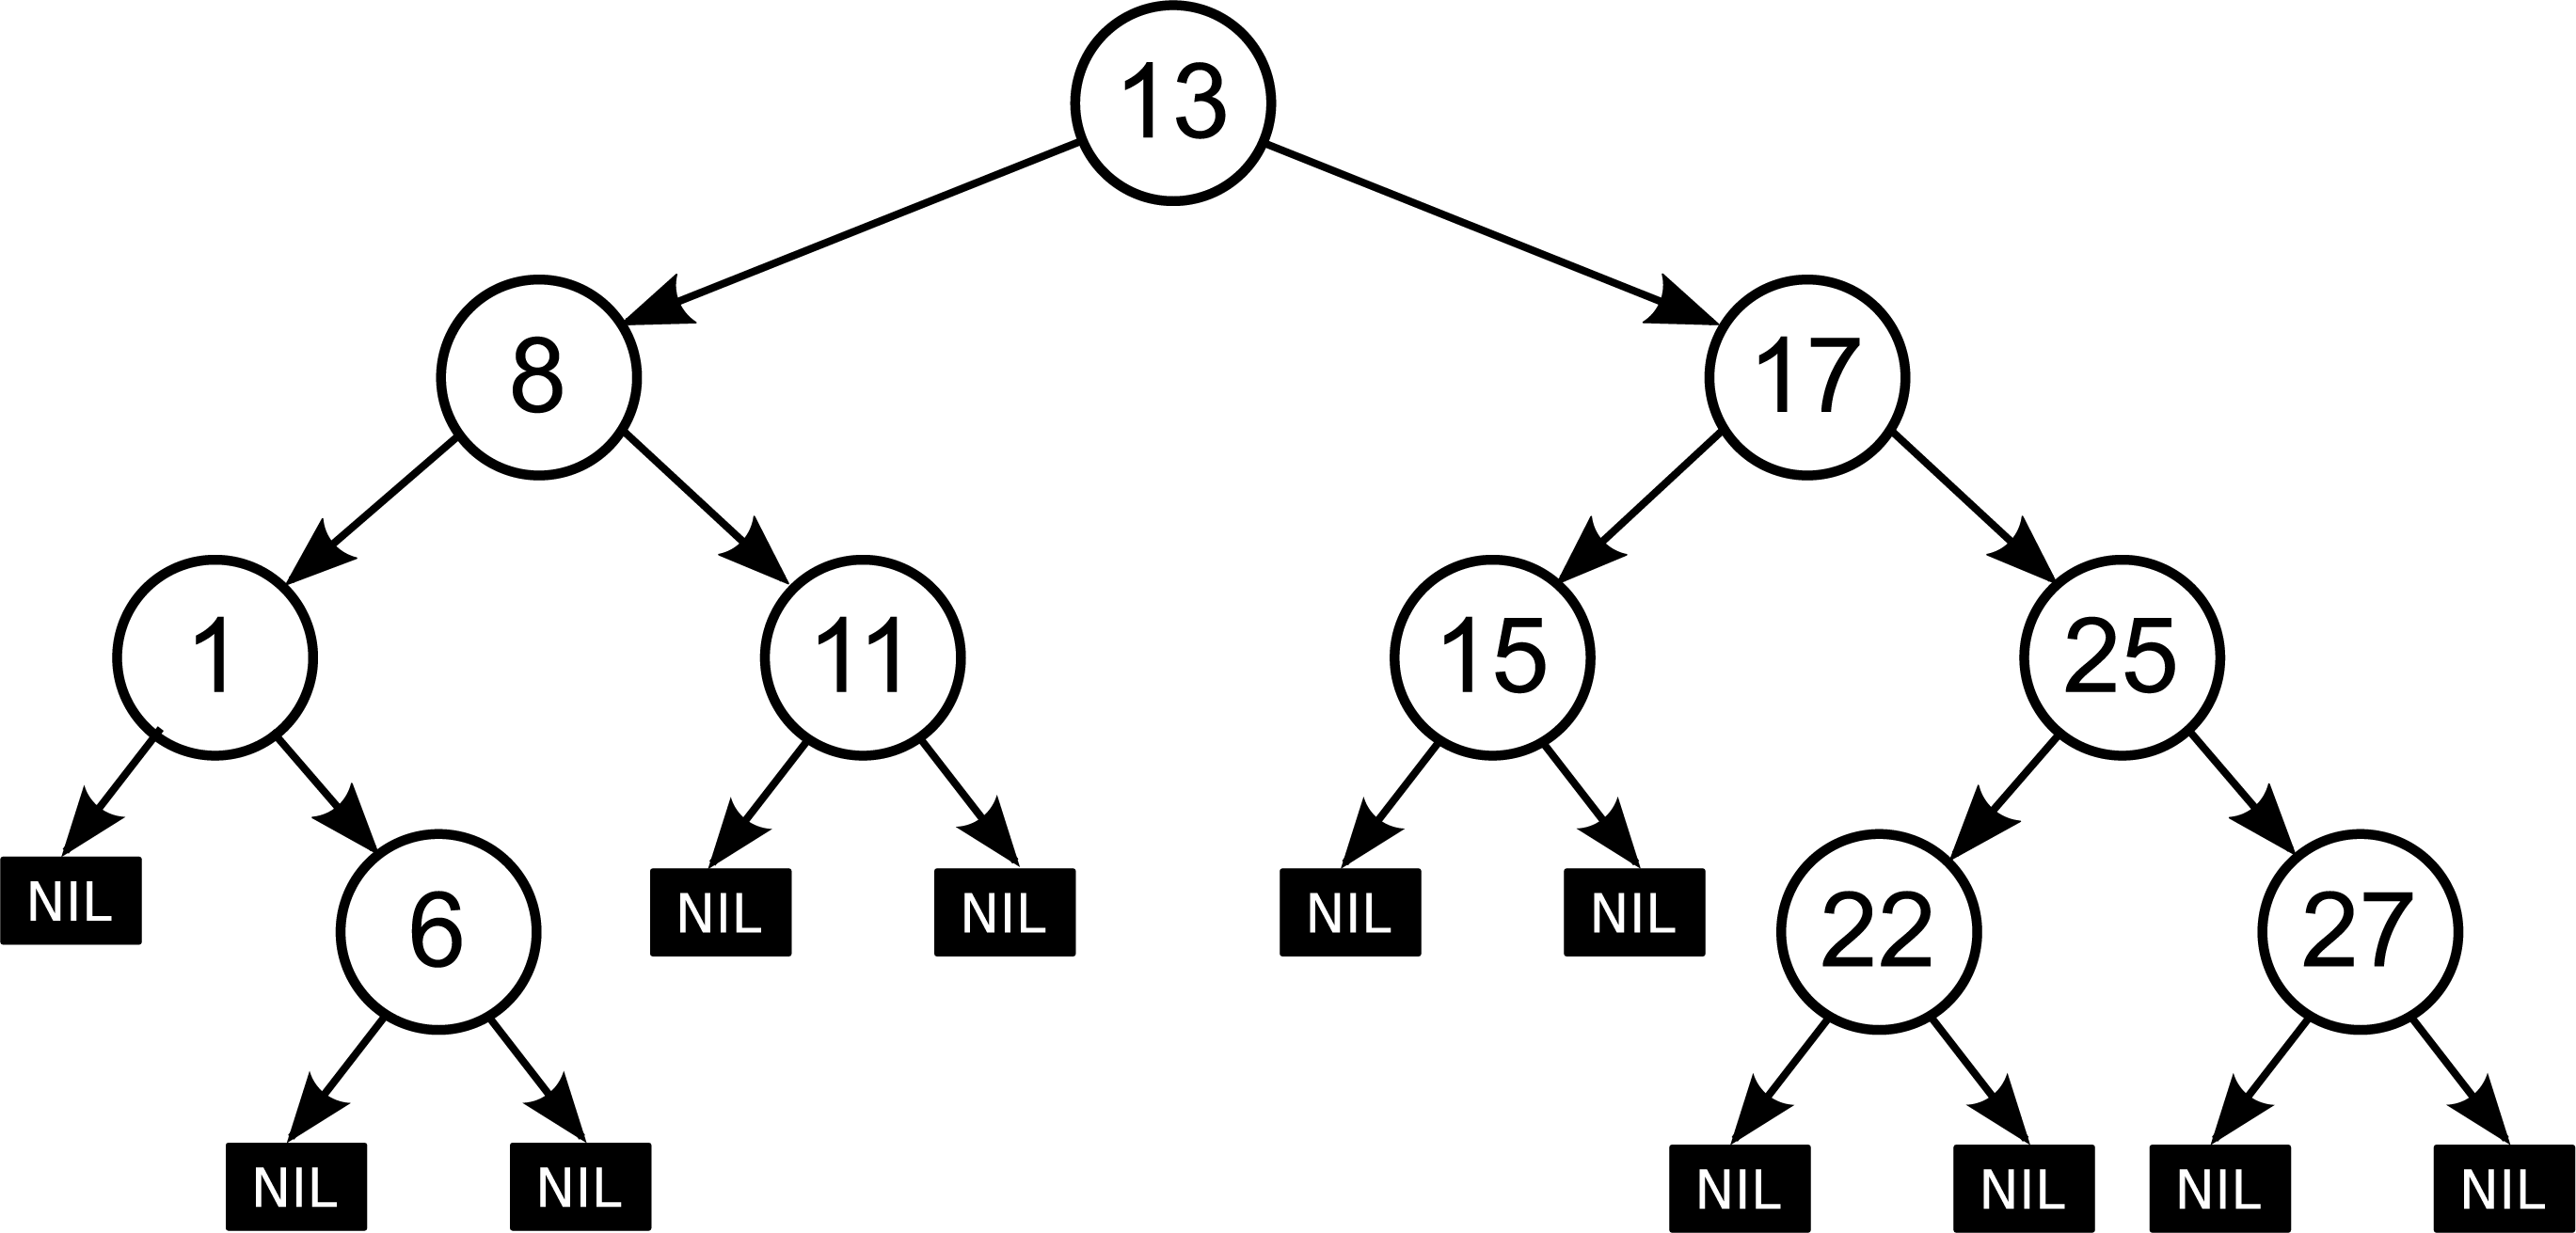
\includegraphics[width=\textwidth]{img/binary_tree.png}}
\only<2>{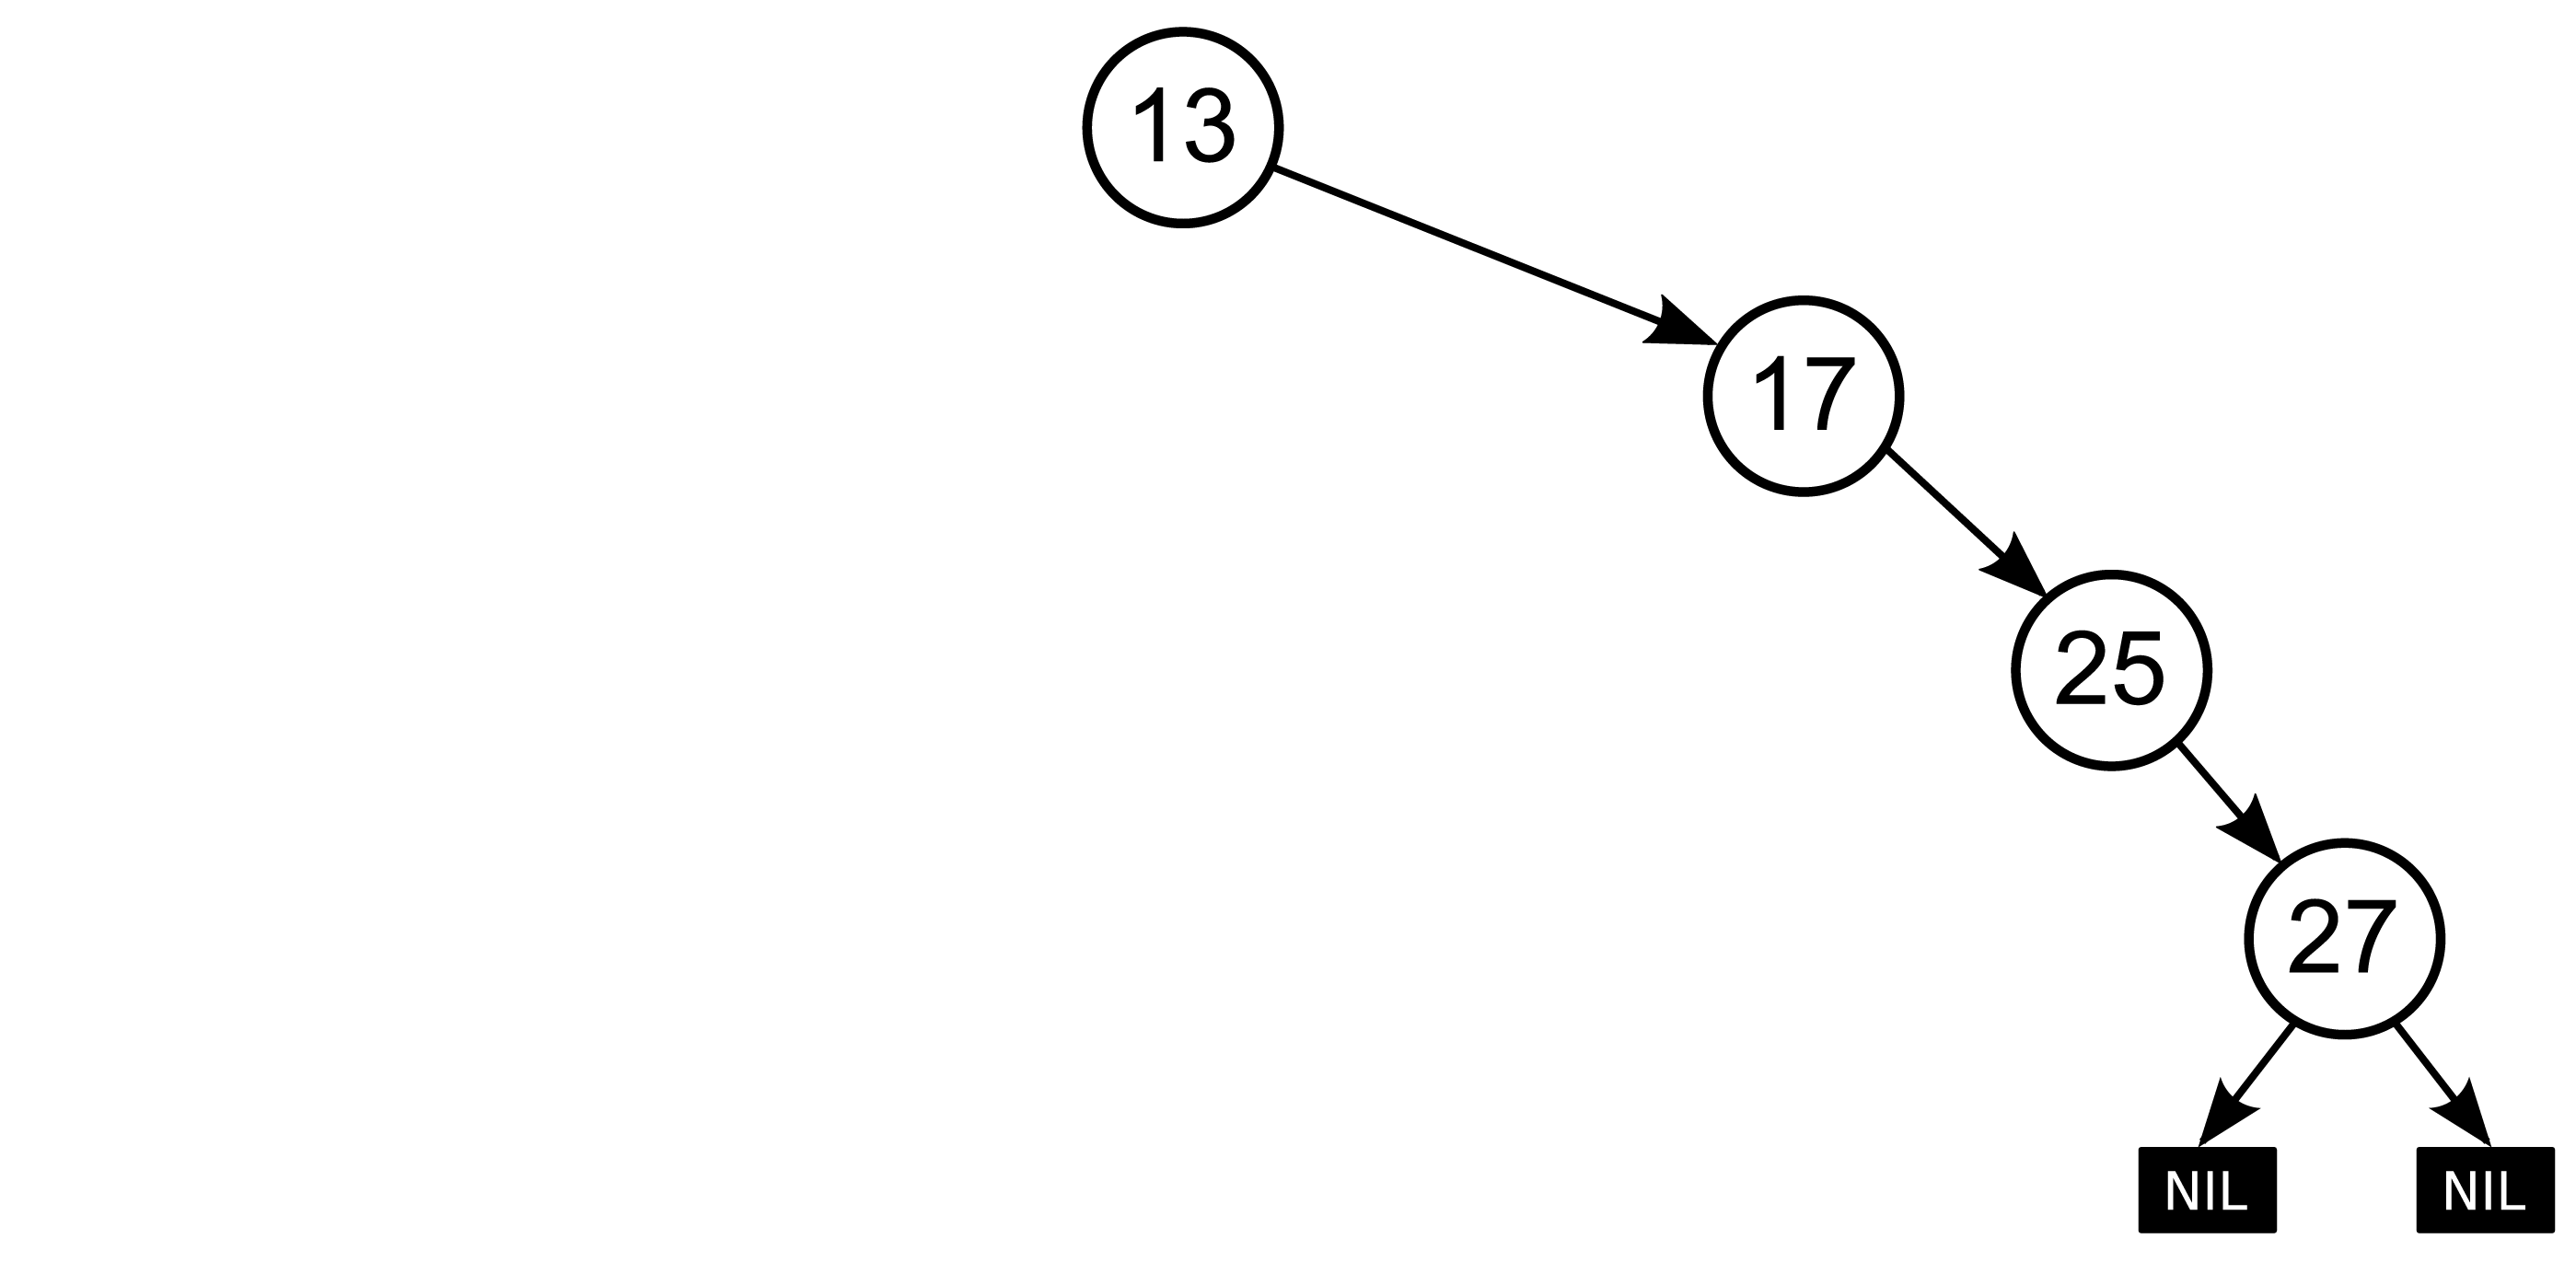
\includegraphics[width=\textwidth]{img/binary_tree_unbalanced.png}}
\only<3>{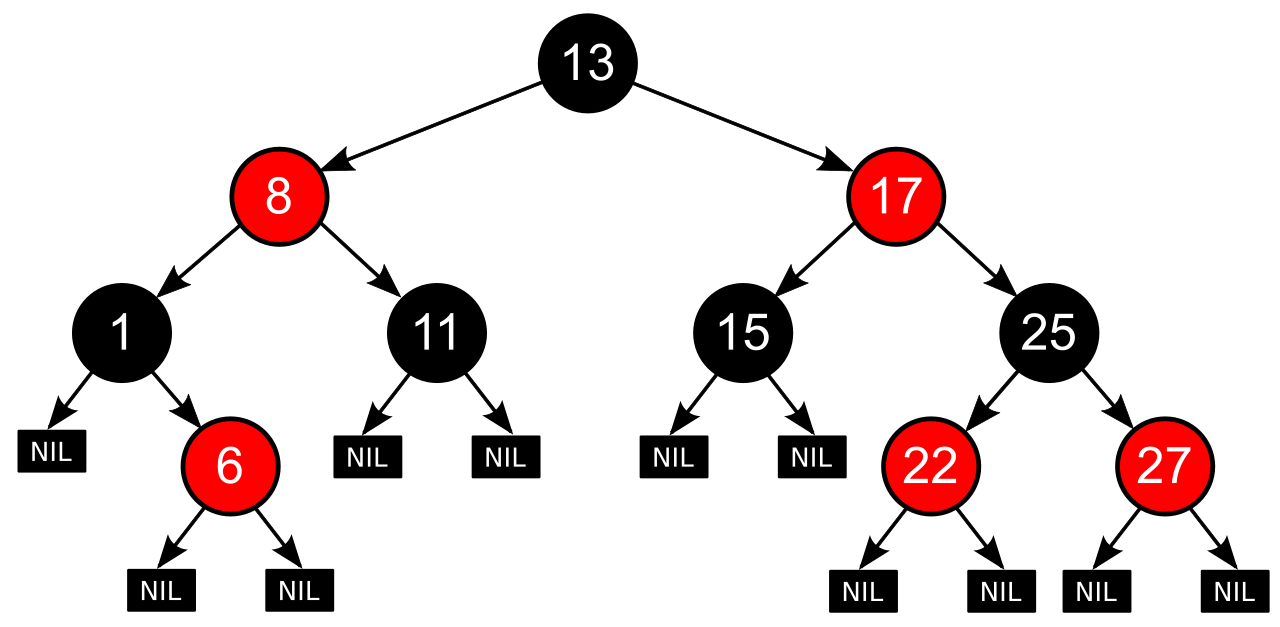
\includegraphics[width=\textwidth]{img/rbtree.png}}
\end{columns}
\end{frame}

\begin{frame}[standout]
  Why verify it?
\end{frame}

\begin{frame}{Red-Black Tree}
\textbf{Properties} \cite{rbtree}
\begin{columns}[T]
\column{0.5\textwidth}
\begin{enumerate}
  \item Each node is either red or black.
  \item All NIL (empty) nodes are considered black.
  \item A red node does not have a red child.
  \item Every path from a given node to any of its descendant NIL nodes goes through the same number of black nodes.
  \only<2>{\item The root is black.}
\end{enumerate}

\column{0.5\textwidth}
\centering
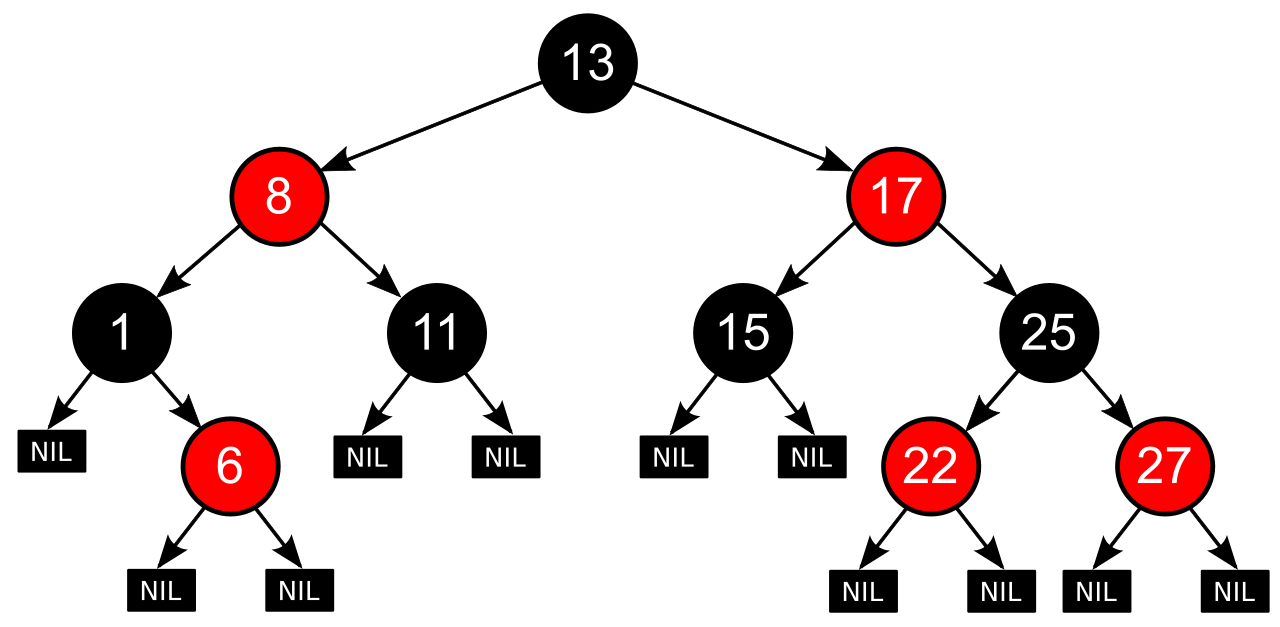
\includegraphics[width=\textwidth]{img/rbtree.png}
\end{columns}
\end{frame}

\begin{frame}{Insertion}
\begin{columns}[T]
\column{0.5\textwidth}
\textbf{Algorithm}
\begin{enumerate}
  \item Recursively descend in tree to correct position
  \only<2>{
    \item Insert a new red node
    \item Recursively go back up and solve all property violations
  }
\end{enumerate}

\column{0.5\textwidth}
\centering
\only<1>{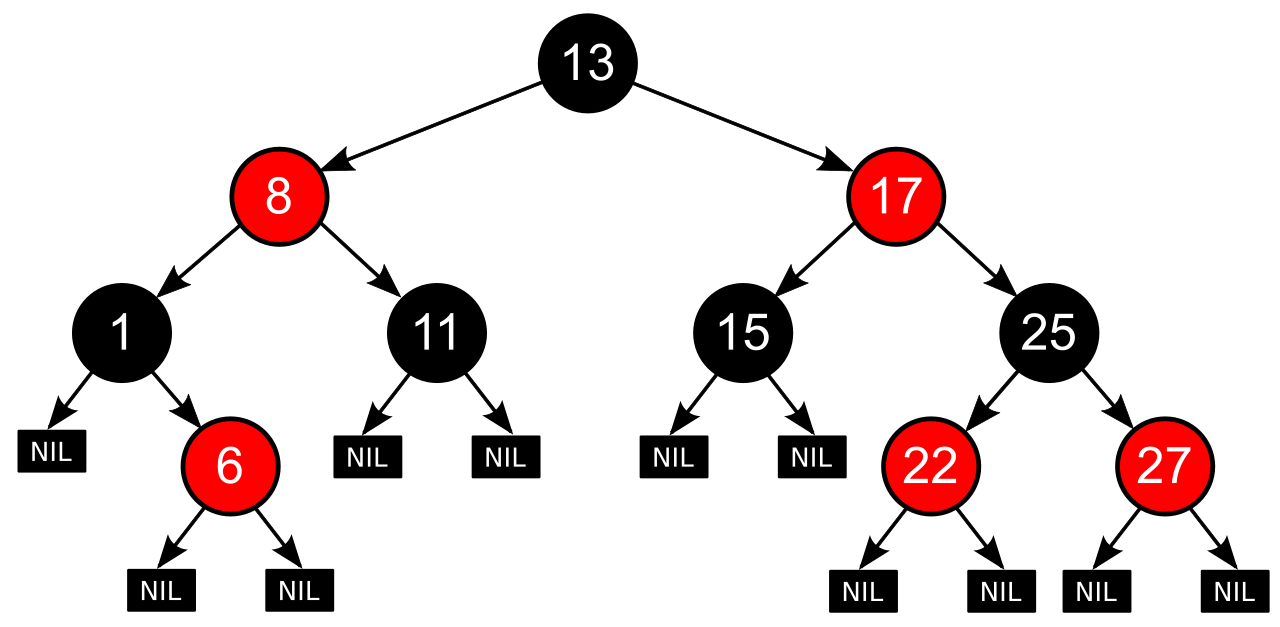
\includegraphics[width=\textwidth]{img/rbtree.png}}
\only<2>{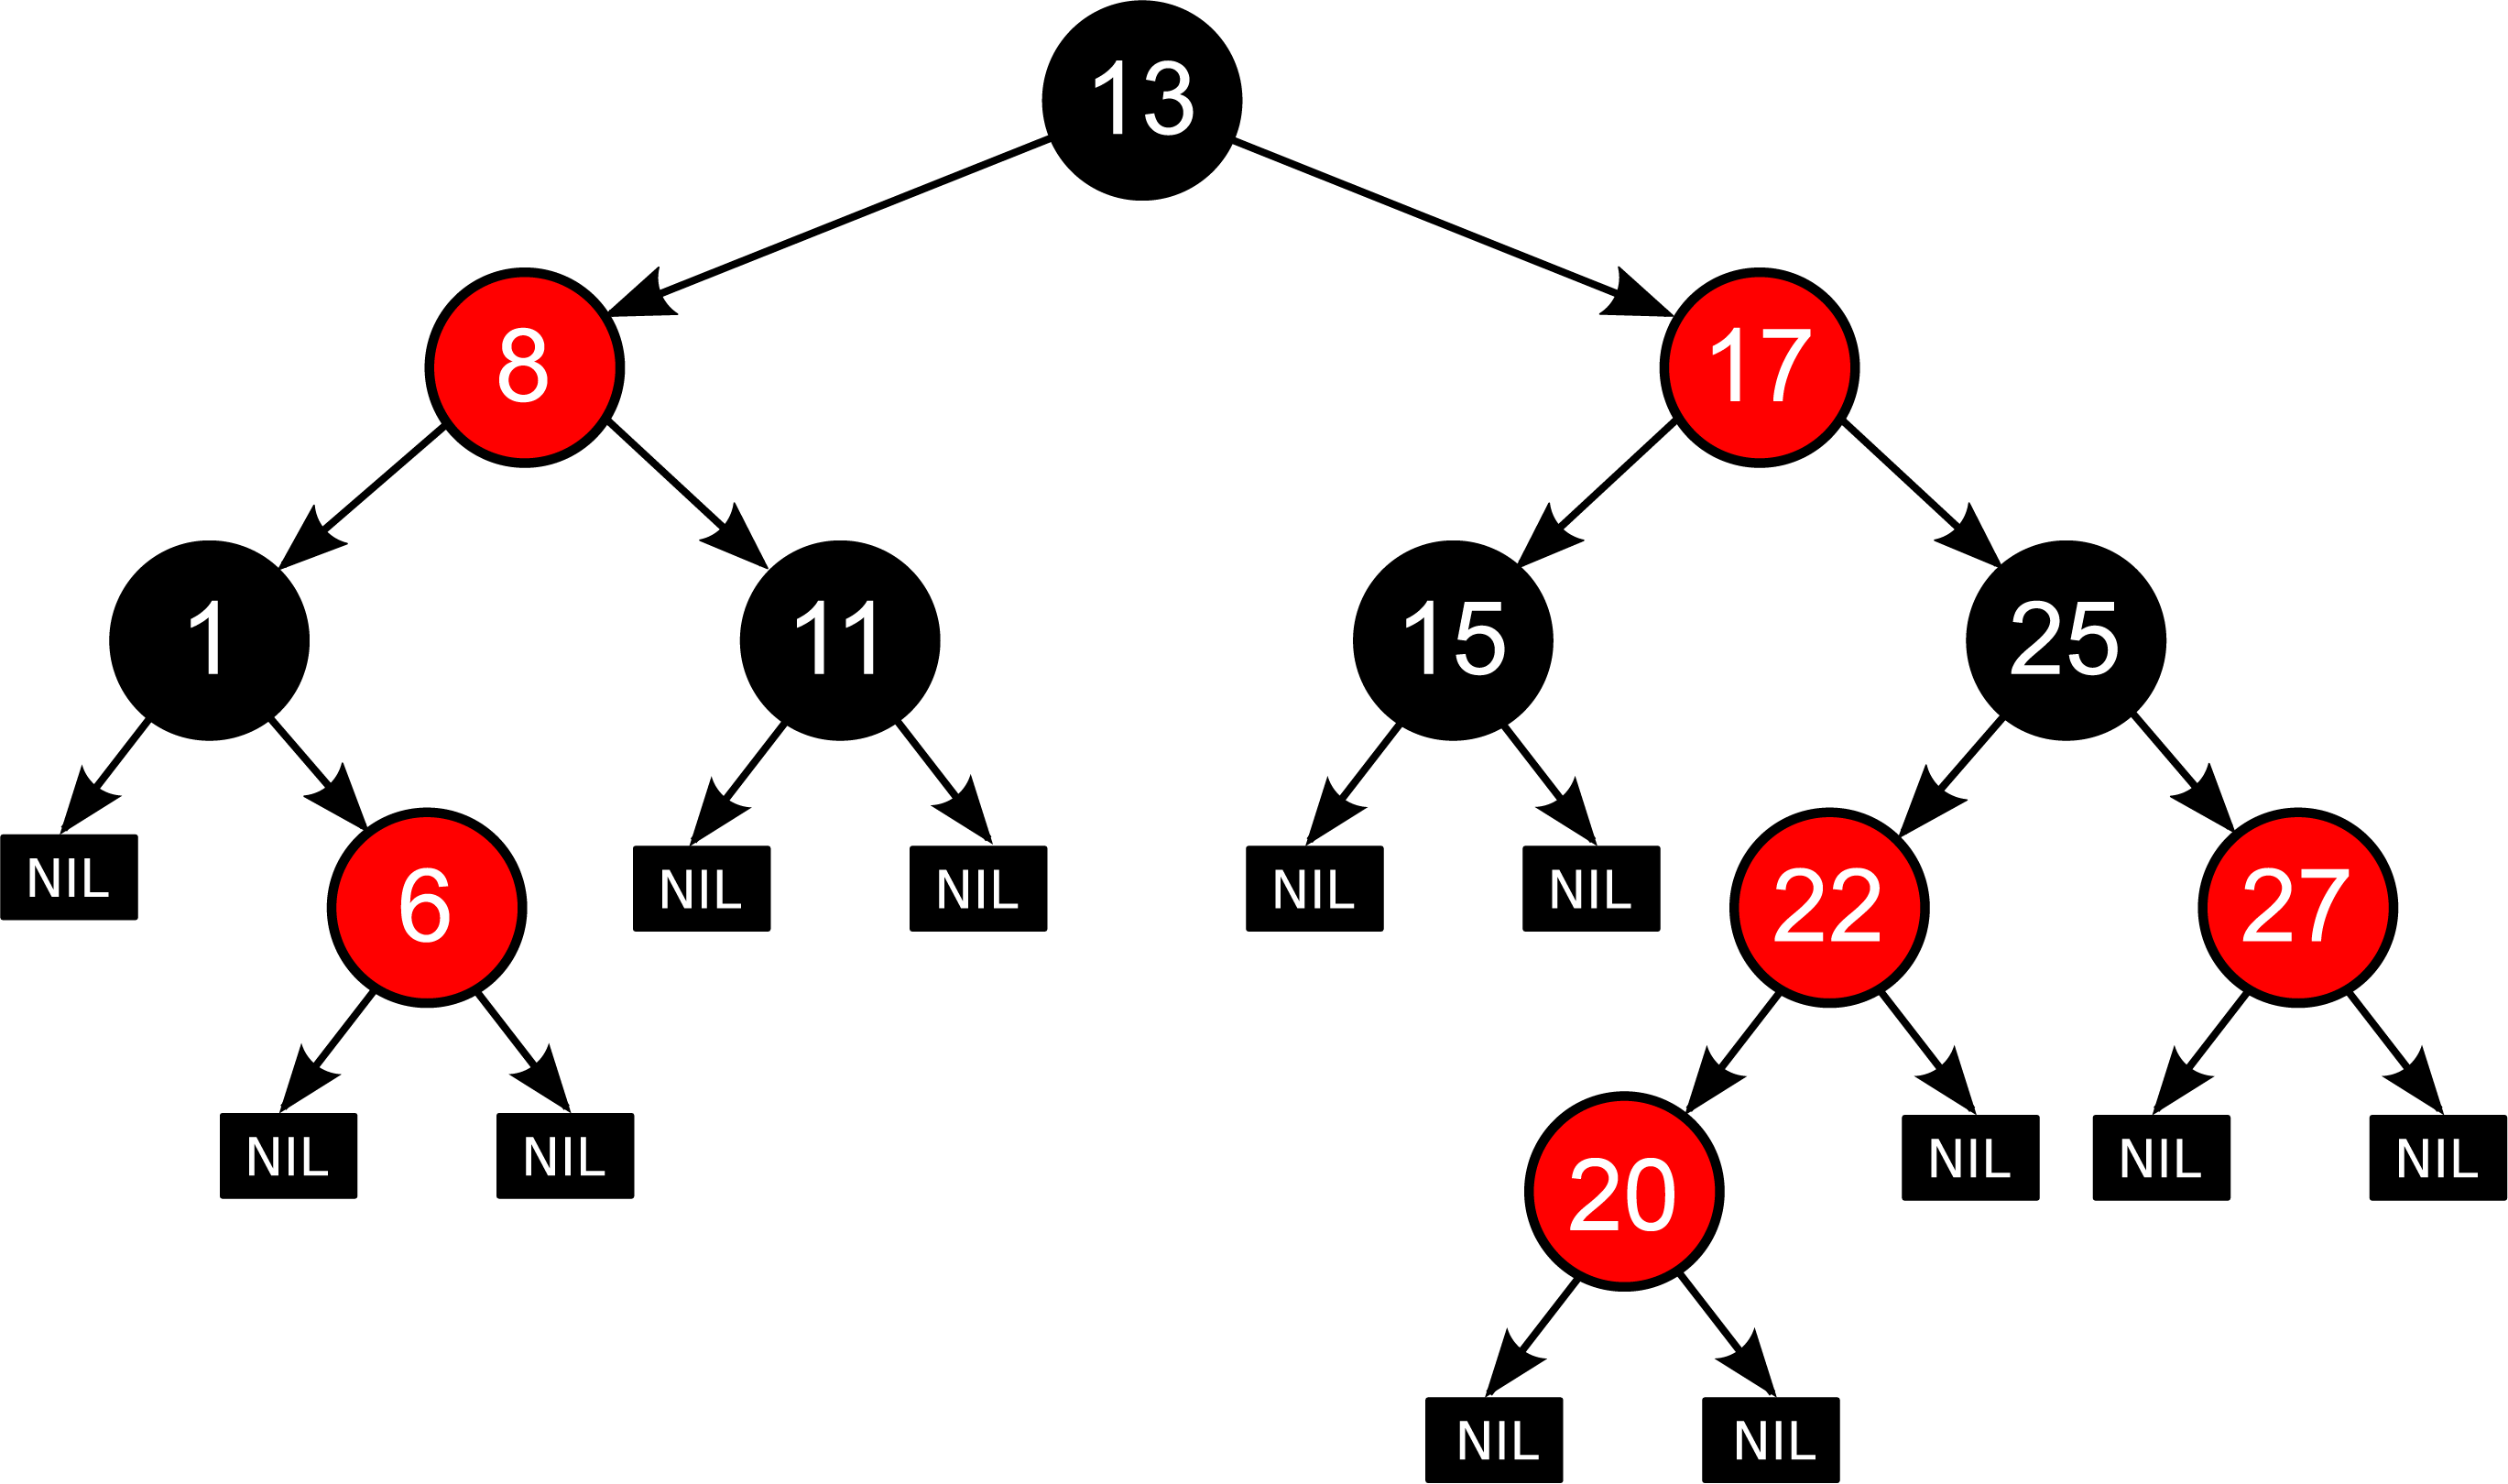
\includegraphics[width=\textwidth]{img/rbtree_insert.png}}
\end{columns}
\end{frame}

\begin{frame}[fragile]{Insertion}
In Scala
\begin{lstlisting}[language=Scala, basicstyle=\footnotesize\ttfamily,]
def ins(x: BigInt, t: Tree): Tree = {
  require(redNodesHaveBlackChildren(t) && blackBalanced(t))
  t match {
    case Empty() => Node(Red(),Empty(),x,Empty())
    case Node(c,a,y,b) =>
      if      (x < y)  balance(c, ins(x, a), y, b)
      else if (x == y) Node(c,a,y,b)
      else             balance(c,a,y,ins(x, b))
  }
} ensuring (res => content(res) == content(t) ++ Set(x)
                 && size(t) <= size(res) && size(res) <= size(t) + 1
                 && redDescHaveBlackChildren(res)
                 && blackBalanced(res))
\end{lstlisting}
\end{frame}

\begin{frame}{Rebalancing}
  \centering
  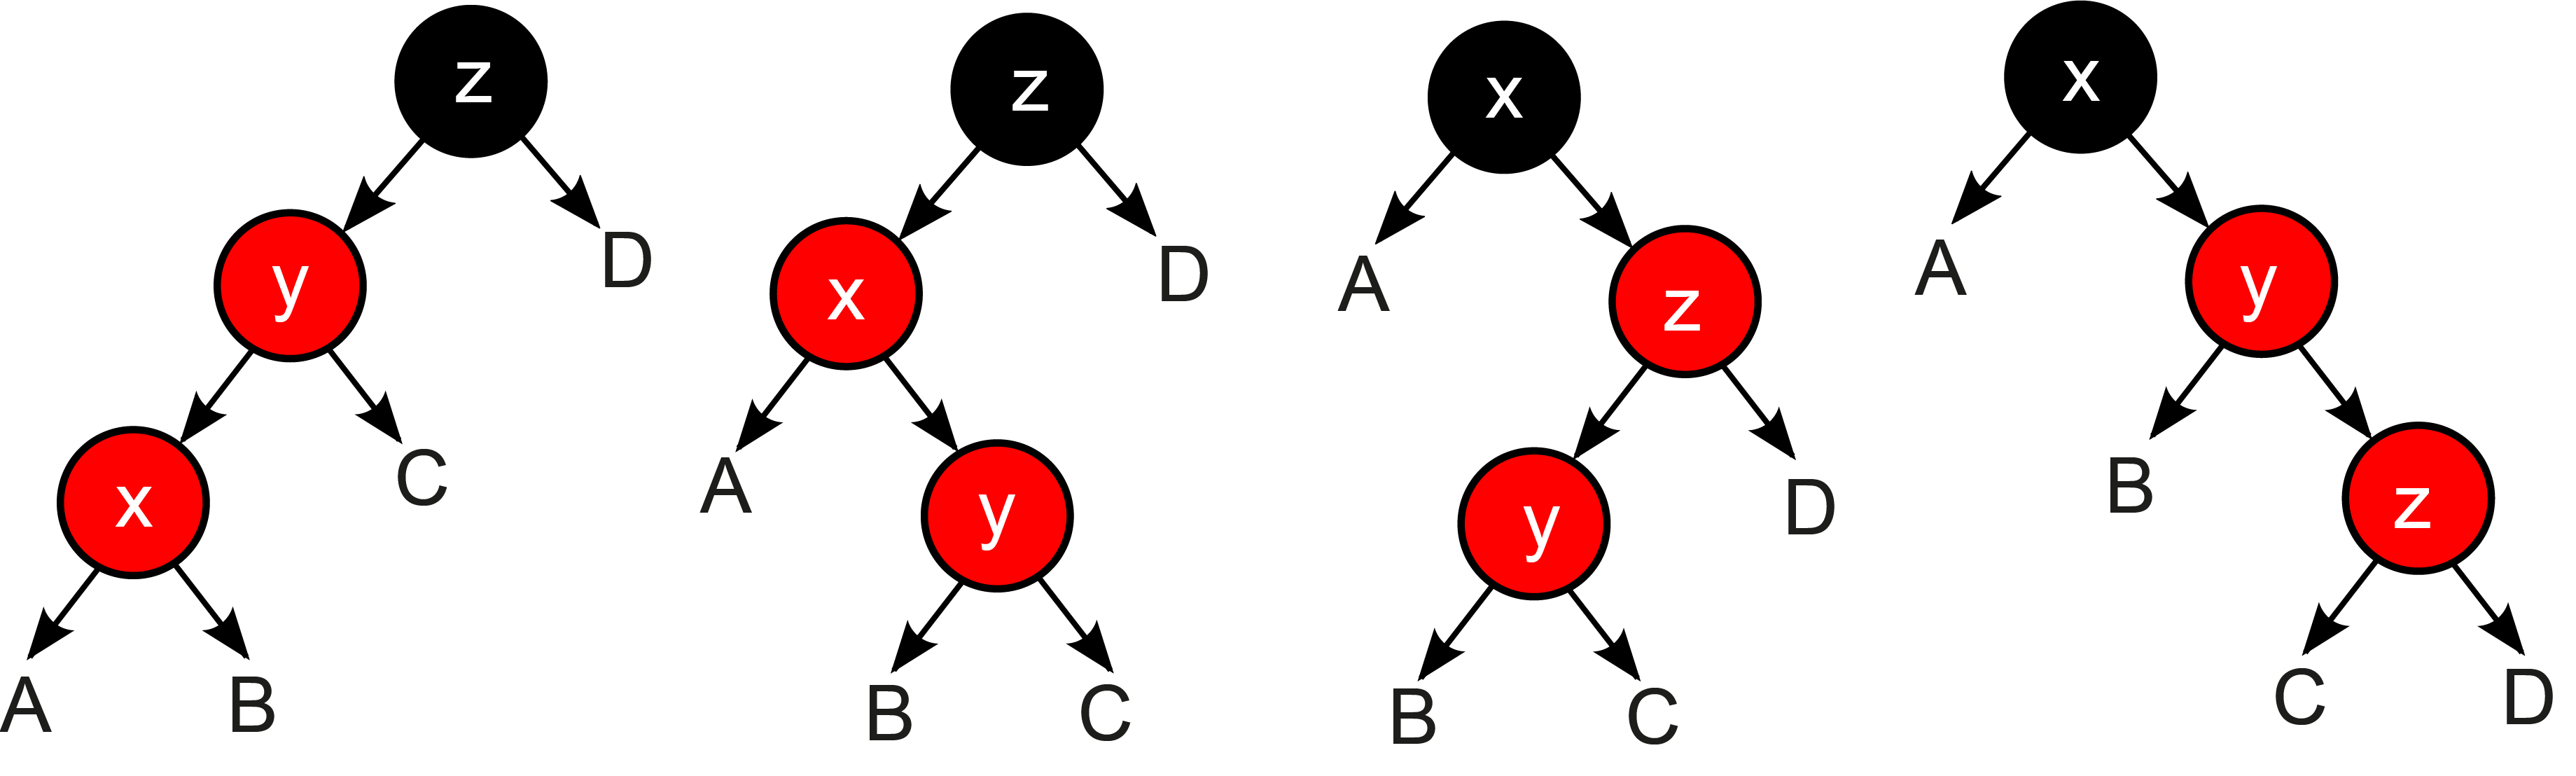
\includegraphics[width=0.8\textwidth]{img/rbtree_cases.png}
  \vfill
  \only<2>{
    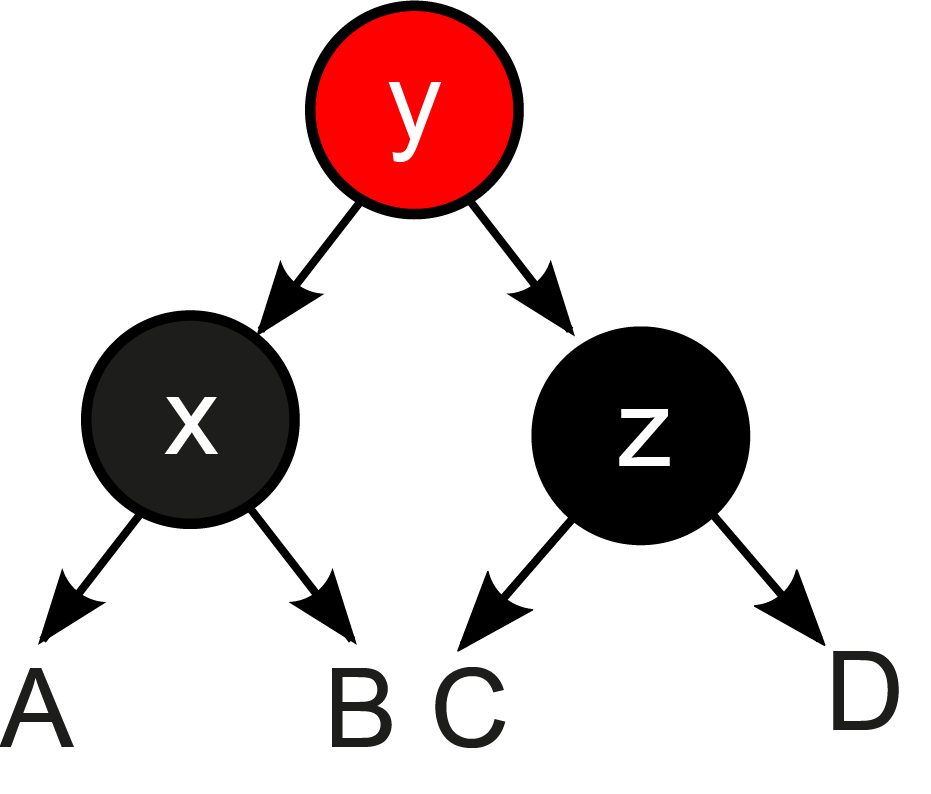
\includegraphics[width=0.3\textwidth]{img/rbtree_solution.png}
  }
\end{frame}

\begin{frame}[fragile]{Rebalancing}
In Scala
\begin{lstlisting}[language=Scala, basicstyle=\footnotesize\ttfamily,]
def balance(c: Color, a: Tree, x: BigInt, b: Tree): Tree = {
    Node(c,a,x,b) match {
      case Node(Black(),Node(Red(),Node(Red(),a,xV,b),yV,c),zV,d) =>
        Node(Red(),Node(Black(),a,xV,b),yV,Node(Black(),c,zV,d))
      case Node(Black(),Node(Red(),a,xV,Node(Red(),b,yV,c)),zV,d) =>
        Node(Red(),Node(Black(),a,xV,b),yV,Node(Black(),c,zV,d))
      case Node(Black(),a,xV,Node(Red(),Node(Red(),b,yV,c),zV,d)) =>
        Node(Red(),Node(Black(),a,xV,b),yV,Node(Black(),c,zV,d))
      case Node(Black(),a,xV,Node(Red(),b,yV,Node(Red(),c,zV,d))) =>
        Node(Red(),Node(Black(),a,xV,b),yV,Node(Black(),c,zV,d))
      case Node(c,a,xV,b) => Node(c,a,xV,b)
    }
  } ensuring (res => content(res) == content(Node(c,a,x,b)))
\end{lstlisting}
\end{frame}

\begin{frame}[standout]
  Why in Rust?
\end{frame}

\begin{frame}{Performance Comparison}
To insert the integers from 1 to 5000 into the implementation takes:
\begin{itemize}
  \item Red-Black Tree in Scala, fully functional, no mutation: 185s
  \only<2>{
    \item  Red-Black Tree in Rust, fully mutable, no allocation
    in rebalancing: \textbf{10ms}
  }
\end{itemize}
\end{frame}

\section{Tool Overview}

\section{Translation}

\subsection{Mutability}

\subsection{Traits to Type Classes}

\section{Conclusions}



\begin{frame}[allowframebreaks]{References}
  \bibliography{bib}
  \bibliographystyle{IEEEtranS}
\end{frame}
